% !TeX spellcheck = es_ANY
% Chapter 1

%\chapter{Chapter Title Here} % Main chapter title
%
%\label{Chapter1} % For referencing the chapter elsewhere, use \ref{Chapter1} 

%----------------------------------------------------------------------------------------

% Define some commands to keep the formatting separated from the content 
\newcommand{\keyword}[1]{\textit{#1}}
%\newcommand{\tabhead}[1]{\textbf{#1}}
%\newcommand{\code}[1]{\texttt{#1}}
%\newcommand{\file}[1]{\texttt{\bfseries#1}}
%\newcommand{\option}[1]{\texttt{\itshape#1}}

%----------------------------------------------------------------------------------------

\section{Introducción}
	La Teor\'ia de la Relatividad General de Albert Einstein fue publicada en 1915, de dicha teor\'ia surgen las ondas gravitacionales como una, entre varias prediciones, las cuales incluyen lentes gravitacionales en donde cuerpos masivos modifican la trayectoria de la luz, as\'i como la dilataci\'on del tiempo. El t\'ermino ``ondas gravitacionales'' fue introduccido por primera vez en una publicaci\'on de Henri Poincaré, 10 a\~nos antes, donde propon\'ia la primera ecuaci\'on para un campo gravitacional invariante ante transformaciones de Lorentz \cite{straumann2012general, bassan2014advanced}. Actualmente se entiende por ondas gravitacionales a las variaciones periódicas de la geometría del espacio-tiempo, y tienen su origen en que la energía y densidad de momento de un campo gravitacional actúan a su vez como fuentes de gravedad \cite{hoyng2006gravitational}. A pesar que han pasado más de 100 años desde la publicación de la teoría, aun hoy en día existen vacíos en el entendimiento y las implicaciones de las ecuaciones de Einstein. Lo anterior se debe en parte a la dificultad de resolver las ecuaciones para situaciones físicas de interés, por ejemplo en el caso de las ondas gravitacionales sólo se pueden resolver analíticamente para campos débiles usando una forma lineal de estas ecuaciones. Los cuales detectaron en 2016 de forma simultánea y por primera vez en la historia de la humanidad una onda gravitacional, lo cual fue reconocido por la comunidad científica en 2017 con el Premio Nobel de Física \cite{brugmann2018fundamentals}.  
	
	Si bien cuales quiera dos objetos con masas desiguales generan ondas gravitacionales al orbitar sobre el centro de masa, la mayor\'ia de campos gravitacionales en el universo son d\'ebiles, entre las pocas escepciones se encuentran los campos cercanos a cuerpos extremadamente masivos, como agujeros negros y estrellas de neutrones, raz\'on por la cual	en la pr\'actica solo las ondas gravitacionales provenientes de cuerpos extremadamente masivos son detectables \cite{straumann2012general}. Esto restringe las fuentes a sistemas binarios de estrellas, agujeros negros y supernovas (siempre que la explosi\'on no sea sim\'etrica). En el caso de los agujeros negros las ondas gravitacionales constituyen una herramienta muy poderosa para su estudio, pues a excepción de su gravedad, y su tamaño, un agujero negro es muy similar a cualquier otro objeto en el universo, bien sea una estrella o un planeta \cite{meier2012black}. Dada la magnitud de la gravedad generada, no es posible que la luz escape de él. Esto da lugar a una superficie invisible, en el caso de encontrarse cerca, es posible detectar un agujero negro pues el paso de este por el firmamento ocultar\'ia las estrellas del fondo. Pero a largas distancias, este efecto es poco apreciable y por ende no es posible observarlos por un instrumento \'optico como un telescopio. Por otro lado, cuando la distancia entre el observador y un agujero negro es muy grande, sus efectos gravitacionales son poco distintos a los presentados por un objeto con la misma masa, pero un volumen considerablemente mayor, pues a largas distancias ambas serán aproximadamente masas puntuales \cite{meier2012black}.
	
	Los esfuerzos por detectar ondas gravitacionales empezaron con el uso de barras resonantes por el f\'isico estadounidense Joe Weber en 1965 \cite{weber1967gravitational, bassan2014advanced}. Por varias d\'ecadas, la tecnolog\'ia, la sensibilidad y la extensi\'on de las barras de Weber mejor\'o, a tal punto de formar la primera red de observaci\'on global ondas gravitacionales. Sin embargo el acoplamiento entre materia y ondas es tan peque\~no, que en el caso de la detecci\'on de ondas gravitacionales existen factores que en otros contextos no seri\'an tan relevantes, como es el caso de las fuentes de ruido, entre los cuales se encuentran: t\'ermico y s\'ismico, \textit{shot noise} y su frecuencia \cite{bassan2014advanced}. Si bien los detectores de interferometr\'ia no estaban excentos de estas fuentes de ruido, presentan mayor sensitividad que las barras resonantes, por lo cual hoy en d\'ia son los m\'as usados. Siendo los dos m\'as representativos LIGO (\textit{Laser Interferometer Gravitational-Wave Observatory} por sus siglas en ingl\'es) y Virgo, en Estados Unidos y Europa, correspondientemente \cite{abbott2009ligo, acernese2008status, bassan2014advanced}.
	
	\begin{figure}[h]
		\centering
		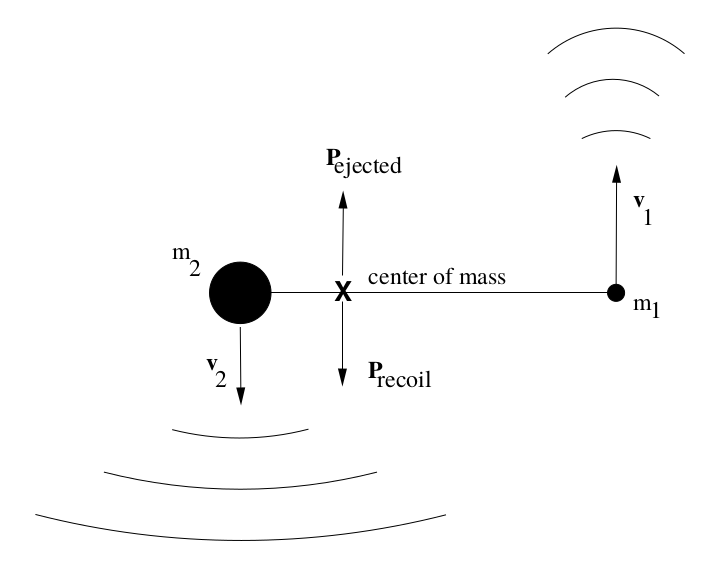
\includegraphics[width=0.6\linewidth]{Figures/binarySystem}
		\caption{Sistema binario con cuerpos de masas $m_1$ y $m_2$ ($m_2 > m_1$), emisor de ondas gravitacionales \cite{hughes2005black}.}
		\label{fig: binary}
	\end{figure}
	
	En el caso de un sistema binario como el de la \autoref{fig: binary}, visto desde la gravitación universal de Newton, se tendría como solución a las ecuaciones de movimiento trayectorias elípticas en concordancia con las leyes de Kepler. Sin embargo, al considerar la Relatividad General, se producirán ondas que llevan energ\'ia y momento \cite{hughes2005black, hoyng2006gravitational, brugmann2018fundamentals}. Esto ocasiona que poco a poco la \'orbita decaiga y los dos objetos se fusionen en un \'unico cuerpo. En el momento en que tiene lugar la fusi\'on de los cuerpos la amplitud de la onda aumenta considerablemente. Un fen\'omeno que se ha comprendido durante bastante tiempo, sin embargo sus implicaciones han sido poco estudiadas, son aquellas que se relacionan con el momento lineal que lleva la onda. Esto implica que al aumentar la amplitud de la onda con la fusi\'on, tambi\'en lo hace el momento lineal de la onda ($\mathbf{P}_{\text{ejected}}$), por lo cual la fusi\'on ocasiona que el centro de masa se mueva en direcci\'on opuesta con momento $\mathbf{P}_{\text{recoil}}$ para conservar el momento del sistema. A este movimiento del centro de masa se le conoce con el nombre de retroceso o patada (\textit{recoil} o \textit{kick}) \cite{hughes2005black} y fue descrito por Bonnor y Rotenberg en 1966 \cite{bonnor1966gravitational}.
	
	En la mayoría de los casos el decaimíento de un sistema binario es tan lento que sucede en escalas de millones o billones de años, pero para el caso de los agujeros negros y estrellas de neutrones las ondas gravitacionales son de vital importancia. En estos mismos casos los campos gravitacionales son fuertes, por lo cual no es posible usar las soluciones analíticas a las ecuaciones de Einstein, es entonces donde los métodos numéricos, aplicados a simulaciones computacionales permiten obtener soluciones a las ecuaciones de Einstein y de esta forma proveer un marco de referencia teórico para el estudio de agujeros negros binarios, estrellas de neutrones y ondas gravitacionales en general \cite{brugmann2018fundamentals}.
%	Una forma de entender c\'omo sucede este fen\'omeno, es usando un sistema con masas desiguales. Se puede considerar dos cuerpos, uno con masa $m_1$ y otro con masa $m_2$, donde $m_2 > m_1$. En el caso cl\'asico, donde no existe ning\'un efecto nuevo, se tiene que el centro de masa orbitar\'ia alrededor de un c\'irculo. Sin embargo, cuando se tiene una onda que lleva energ\'ia y momento angular, se tiene que los cuerpos seguir\'ian una trayector\'ia en espiral, por lo cual al considerar toda una \'orbita ($\mathcal{O}$) se tendr\'ia que:
%	
%	\begin{equation}
%		\int\limits_{\mathcal{O}_1} m_1\vec{v}_1dl \neq \int\limits_{\mathcal{O}_2} m_2\vec{v}_2dl 
%	\end{equation}	
	
\section{Objetivo general}
%	Poner en funcionamiento el calorímetro 2277 Thermal Activity Monitor con el que se cuenta, en funcionamiento y adicionalmente calibrar el equipo para su uso en las investigaciones activas del grupo \groupname.
		
\section{Objetivos específicos}
%	\begin{itemize}
%		\item Ensamblar el equipo 2277 Thermal Activity Monitor.
%		\item Realizar el cableado y conexiones electrónicas pertinentes al mismo.
%		\item Calibración eléctrica, determinación de las señales de entrada y salida, flujo de las bombas hidráulicas y temperatura del baño.
%		\item Calibración química, determinación de la entalpía molar, energía libre de Gibbs, entropía, y constante de equilibrio, del acomplejamiento del catión bario con éter 18-corona-6.
%	\end{itemize}
	
\section{Metodología}
	Las simulaciones ser\'an realizadas en el cluster de la universidad (HPC) con el fin de paralelizar procesos, de forma que a haciendo uso de sus recursos se minimice el tiempo de simulación a fin de lograr la mayor cantidad de simulaciones posibles con el fin de obtener una cantidad significativa de datos de validación.
	
\section{Consideraciones éticas}
	Se manejará un repositorio de uso privado a través de Github en donde se encontrar\'an los códigos implementados en cada parte del proceso, junto con los resultados obtenidos, de forma que se asegure la reproducibilidad del modelo hallado, al mismo tiempo que se permita el seguimiento del uso de recursos. Adem\'as al mantener la informaci\'on abierta se asegura que no se están utilizando resultados obtenidos por otros investigadores de forma directa.
	
\section{Cronograma}
	\begin{table}[h]
		\centering
		\caption{Cronograma de actividades}
		\label{tb: cronograma}
		\footnotesize
		\begin{tabular}{|c|c|c|c|c|c|c|c|c|c|c|c|c|c|c|c|c|}
			\hline
			\rowcolor[HTML]{C0C0C0} 
			\cellcolor[HTML]{C0C0C0}                                       & \multicolumn{16}{c|}{\cellcolor[HTML]{C0C0C0}\textbf{Semana}} \\ \cline{2-17} 
			\rowcolor[HTML]{EFEFEF} 
			\multirow{-2}{*}{\cellcolor[HTML]{C0C0C0}\textbf{Actividades}} & \textbf{1} & \textbf{2} & \textbf{3} & \textbf{4} & \textbf{5} & \textbf{6} & \textbf{7} & \textbf{8} & \textbf{9} & \textbf{10} & \textbf{11} & \textbf{12} & \textbf{13} & \textbf{14} & \textbf{15} & \textbf{16} \\ \hline
			\cellcolor[HTML]{EFEFEF}
			\textbf{Revisión bibliográfica} & x & x & x & & & & x & x & x & x & & & & x & x & x \\ \hline
			\cellcolor[HTML]{EFEFEF}\textbf{Revisión de manuales} & x & x & x & x & & & & & & & & & & & & \\ \hline
			\cellcolor[HTML]{EFEFEF}\textbf{Ensamble del equipo} & x & x & x & x & & & & & & & & & & & & \\ \hline
			\cellcolor[HTML]{EFEFEF}\textbf{Cableado y electrónica} & & & x & x & x & x & & & & & & & & & & \\ \hline
			\cellcolor[HTML]{EFEFEF}\textbf{Calibración eléctrica} & & & & & & x & x & x & & & & & & & & \\ \hline
			\cellcolor[HTML]{EFEFEF}\textbf{Calibración química} & & & & & & & & & x & x & x & x & & & & \\ \hline
			\cellcolor[HTML]{EFEFEF}\textbf{Análisis de datos} & & & & & & & & & & & x & x & x & & & \\ \hline
			\cellcolor[HTML]{EFEFEF}\textbf{Elaboración del documento} & & & & & & & x & x & x & x & & & & x & x & x \\ \hline
			\cellcolor[HTML]{EFEFEF}\textbf{Presentación del proyecto} & & & & & & & & & & & & & & & & x \\ \hline
		\end{tabular}
	\end{table}